\documentclass[tikz,border=10pt]{standalone}
\begin{document}
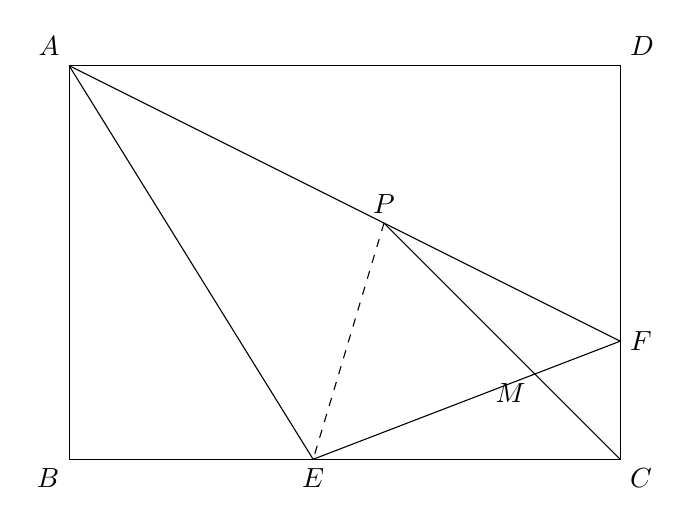
\begin{tikzpicture}
    \coordinate (A) at (0, 5);
    \coordinate (B) at (0, 0);
    \coordinate (C) at (7, 0);
    \coordinate (D) at (7, 5);
    \coordinate (E) at (3.1, 0);
    \coordinate (F) at (7, 1.5);
    \coordinate (P) at (4, 3);
    \coordinate (M) at (5.92, 1.08);

    \draw (A) -- (B) -- (C) -- (D) -- (A);
    \draw (A) -- (E);
    \draw (A) -- (F);
    \draw (E) -- (F);
    \draw[dashed] (P) -- (E);
    \draw (C) -- (P);

    \node[above left] at (A) {$A$};
    \node[below left] at (B) {$B$};
    \node[below right] at (C) {$C$};
    \node[above right] at (D) {$D$};
    \node[below] at (E) {$E$};
    \node[right] at (F) {$F$};
    \node[above] at (P) {$P$};
    \node[below left] at (M) {$M$};
\end{tikzpicture}
\end{document}
